\documentclass[a4paper,cleardoubleempty,BCOR1cm]{scrbook}
% use to waste space:
% \documentclass[12pt,a4paper]{article}

% if you have this style and like it.
%\documentclass{acmsiggraph}
%\documentclass[review]{acmsiggraph}      % review
%\documentclass[widereview]{acmsiggraph}  % wide-spaced review
%\documentclass[preprint]{acmsiggraph}    % preprint

% define a \comment{this is a comment which can have linebreaks in it}
\newcommand{\comment}[1]{}
% \newcommand{\todo}[1]{\marginpar{\bf{#1}}}
\newcommand{\todo}[1]{{\color{red}\bf{TODO: #1}}}

\usepackage{mathptmx}
\usepackage[pdftex]{graphicx}
\usepackage[pdftex]{color}
\definecolor{rot}{RGB}{165,30,55} %rote Farbe
\graphicspath{{./images/}}
\usepackage{parskip}
\usepackage{amsmath}
\usepackage{dsfont}
\usepackage{pxfonts}

\usepackage[T1]{fontenc}
\usepackage{textcomp}
\usepackage{acronym}
\usepackage[font=small,labelfont=bf]{caption}

% comment these two lines out if you don't want minion/myriad fonts.
% \usepackage[minionint,mathlf]{MinionPro}
% \renewcommand{\sfdefault}{Myriad-LF}
%\usepackage{Myriad}

% no page number on float pages, fixes problems with overlarge diagrams.
\usepackage{fancyhdr}
\pagestyle{fancy}
%\lhead{}
%\chead{}
%\rhead{}
%\lfoot{}
\fancyhf{}
\fancyhead[EL]{\nouppercase{\leftmark}}
\fancyhead[OR]{\nouppercase{\rightmark}}
\cfoot{}
%\fancyfoot[EL]{\iffloatpage{}{\thepage}}
%\fancyfoot[OR]{\iffloatpage{}{\thepage}}
\fancyfoot[EL]{\thepage}
\fancyfoot[OR]{\thepage}
\renewcommand{\headrulewidth}{0pt}
\renewcommand{\footrulewidth}{0pt}

%\usepackage{natbib}		% textual referencing
%\usepackage[numbers,super]{natbib}	% nice superscripts
%\bibliographystyle{chicago}	% shitty
\bibliographystyle{alpha}	% abbr names and year in \cite
%\bibliographystyle{agsm}	% australian, need natbib
%\bibliographystyle{kluwer}	% need natbib
%\bibliographystyle{apalike}	% lengthly
%\bibliographystyle{abbrv}	% minimal?

% use for german line breaking:
%\usepackage[ngerman]{babel}
\usepackage[T1]{fontenc}
\usepackage[utf8x]{inputenc}

% avoid us-style text color destruction:
\frenchspacing
\usepackage{microtype}

% have a nice framebox with border directly around the image:
\fboxsep 0pt
\newcommand{\fimg}[2]{\fbox{\includegraphics[width=#1]{#2}}}

\usepackage{theorem}
\theorembodyfont{\upshape}
\newtheorem{definition}{Definition}

\usepackage{listings}
\lstset{numbers=left, numberstyle=\tiny, basicstyle=\tiny, language=C++}
\usepackage[boxruled]{algorithm2e}
%\usepackage{hyperref}
\usepackage{url}
\usepackage{subfig}

\def\code#1{{\tt{#1}}}



\title{Thesis Template}
\author{My Name \thanks{e-mail: my.name@uni-tuebingen.de}}
\date{\today}
\begin{document}

\begin{tabular}{lr}
% 
\includegraphics[width=0.5\linewidth]{logo_sw} % logo bw
 
\includegraphics[width=0.5\linewidth]{UT_WBMW_Rot_4C} % logo red
 & \hspace{0.2\linewidth}
 \parbox{0.5\linewidth}{
   \large\bf\textsf{\color{rot}{Mathematisch-\\Naturwissenschaftliche\\Fakultät\\\\}}
   \hspace{-.144cm}\normalsize\textsf{\color{rot}{Computergrafik}}
   \vspace{0.6cm}
 }
\end{tabular}

\vspace*{10ex}
Masterarbeit

{\huge\bf\textsf{Pretty Planes and ugly toilets}}

\vspace*{30ex}

Eberhard Karls Universität Tübingen\\
Mathematisch-Naturwissenschaftliche Fakultät\\
Wilhelm-Schickard-Institut für Informatik\\
Computergrafik\\
Denis Jan Heid,~ \verb+denis.heid@student.uni-tuebingen.de+,~ 2019

\vspace*{5ex}

\begin{tabular}{@{}l@{\hspace{2em}}l}
  Bearbeitungszeitraum:& Januar 2019-Juli 2019\vspace*{5ex} \\
  Betreuer/Gutachter:& Prof. Dr. Hendrik Lensch, Universität Tübingen\\
  Zweitgutachter:& Prof. Dr. Andreas Schilling, Universität Tübingen
\end{tabular}

\thispagestyle{empty}
\newpage

\chapter*{Selbstst\"andigkeitserkl\"arung}
Hiermit versichere ich, dass ich die vorliegende Masterarbeit selbst\"andig und
nur mit den angegebenen Hilfsmitteln angefertigt habe und dass alle Stellen,
die dem Wortlaut oder dem Sinne nach anderen Werken entnommen sind,
durch Angaben von Quellen als Entlehnung kenntlich gemacht worden sind.
Diese Masterarbeit wurde in gleicher oder \"ahnlicher Form in keinem anderen
Studiengang als Pr\"ufungsleistung vorgelegt.

\vspace*{8ex}
\hrule
\vspace*{2ex}
Denis Heid (Matrikelnummer 3827662), \today



\chapter*{Abstract}
points2mesh, the happening

\chapter*{Auszug}
braucht man doch auch in deutsch?

\chapter*{Acknowledgments}
Th\"anks fabi. Lensch ist nice von dir dass ich hier das machen kann.
Schilling fuer zweitkorrektur.
Th\"anks rike fuer moralische unterstuetzung


\tableofcontents

%% braucht kein Mensch ...
%\listoffigures
%\listoftables


% write content here or...
\chapter{Introduction}
\todo{watertight meshes}
\todo{ in case, incomplete training, mehr optimierung}
  For humans to interact with the world depends on many variables. 
  An important aspect is to recognize, analyze, and estimate the position,
  as well as the shape of objects positioned in the world around. For many years,
  to this day, artificial agents have been developed and deployed in the real world\cite{1087032,10.1007978-981-13-0224-4_40} 
  to imitate how humans interact with it. Similarly, a robot has to understand its environment
  by analyzing and interpreting its surroundings. Understanding exactly this requires first and 
  foremost prior comprehension of the shape of nearby objects. 
  Similar to general robotic applications, the by now more feasible solution for autonomous driving
  needs analogous information of its obstacles to prevent collisions and thus allow for safe guidance
  through traffic. 
  Typically, objects are recorded in a way, which results in unstructured, three-dimensional point
  cloud data, for example, with the help of range scanners or structured light.


  Though obtaining information about samples of an object already provides a way to process a three-dimensional object;
  still, the preferred way to operate is in the form of surface information like tri-or quad-meshes.
  Transforming such point cloud data into meshes is a prevalent problem in the context of computer vision. Thus, numerous
  methods have been developed, aiming to solve that problem\cite{817351,Jakob2015Instant}.
  However, finding use in applications like autonomous driving, reconstructing watertight meshes is a crucial step. Calculating robust collisions or
  analyzing an object's surface requires such a complete mesh, without holes, or undefined spots on its surface.

  With recent advancements in deep learning and the abundance of readily available data, much work has been poured
  into neural networks which can process the real world robustly. Consequently, solving the same problem of processing 
  unstructured points in three-dimensional space and obtaining polygonal meshes has garnered attention. Though, many methods 
  rely on voxelized data, since neural networks can naturally process structured data better than unstructured spatial data.

  In this work, a novel convolutional neural network configuration is proposed which computes watertight tri-meshes from unstructured point cloud data.
  By deforming an initial base-mesh based on learned tension feature vectors from the data, the network can reliably generate approximations
  even with low-resolution or noisy data. 
  Since this network is the first of its kind, it is essential to assess its capabilities in comparison to the traditional methods. 
  Therefore, part of this work is to identify its strengths and weaknesses and determine where it may find use and how to build upon it.

  \subsubsection*{Chapter revision}
  \todo{ueberarbeiten. ist schon wieder nicht aktuell}
  First, a revision of techniques and methods are described in chapter \ref{sec:background} to lay the groundwork for this thesis. In chapter \ref{sec:relatedwork}, 
  numerous traditional, as well as machine learning based methods, are reviewed, which work on the transformation of three-dimensional data to polygonal
  meshes.
  After that, the graph based neural network \emph{points2mesh} is explained in detail, how it handles and learns from point cloud data but also how
   it deforms a base-mesh to approximate the underlying object represented by the data.
  Then, in chapter \ref{chap:results} based on different configurations for the neural network, an assortment of resulting meshes are presented and
   contrasted to each other.
  Followed by section \ref{chap:evaluation}, a numerical evaluation, and discussion are conducted to assess the capabilities of the network and its 
  varied proposed configurations. By defining a comparable metric for evaluation, related methods achieving similar results can be analyzed and thus 
  measured against each other.
  To conclude, in chapter \ref{sec:outlook}, the thesis is resolved by taking a look at possible ways of expanding on the network and outlining what
   has been achieved.
  

\chapter{Background}
\label{sec:background}

\begin{enumerate}
    \item Convolutional neural network
    \item Semi-Supervised Classification with Graph Convolutional networks
\end{enumerate}
-nearest neighbor search

-whats a graph

-whats a mesh
\section{Machine Learning review}
\todo{different name for section}
- Convolutional neural networks
- graph Convolution
- 

\label{ml_review}

\section{stuff}
\subsection{Weighted reservoir sampling}
\label{subsec:wrs}




\chapter{Related Work}
\label{sec:relatedwork}

Often in computer graphics, it is necessary to process three-dimensional real-world or digital objects for reconstruction, remeshing or analytical applications. There are many ways to acquire data of the surface of such geometry and more so many techniques to transform and augment that data to different representations. This often non-trivial task is crucial to further process the object in question in later stages of their respective pipeline. Over the years many representations of acquisition data formats and transformation methods, as well as target data formats, have accumulated.\\
In this chapter, various of these techniques and data formats are examined, of which some of them are used in this work as a vehicle for a novel data transformation routine.\\
Initially, classical approaches are examined in section \ref{classic_approaches} which do not rely on artificial intelligence or machine learning methods.
With the recent advances in machine learning, and more so deep learning, many new approaches have been developed and thus considered in this work.
Hence, machine learning based methods are reassessed in section \ref{ml_approaches} which rely on distinctive statistical features in their initial data format or the dataset itself, thus allowing for the transformation.
\todo{citations for this stuff?}
\section{Classical approaches}
\label{classic_approaches}
  In this chapter, classical approaches are examined which do not rely on machine
  learning to transform data of objects from one format to another. 

  In general, a three-dimensional object may be specified by its representation of the
  surface. This representation varies from unstructured point cloud data in three-dimensional space
  to a graph-based representation like triangle-/ or quad-meshes and even poly meshes
  with more than four neighbors per node. Information on the object's surface may also be described
  by three-dimensional discrete scalar field (~Voxels~).  Often the information on an object's
  surface is only partially defined, where some information may be missing. 
  This can be due to acquisition methods, where parts of the object are partially 
  concealed or recorded from insufficient many sides, or that information is not available.

  Starting from these representations of an object's surface, there are many methods 
  of transformation to reach another state of representation. 
  Transforming the data not only makes further processing easier
  but rather during their process, more data on the surface is 
  computed based on the given input data.

  This task is non-trivial since, from one representation of an object's
  surface, many reconstructions in the form of another representation 
  are possible. The amount of data of the object's surface can never
  be entirely perfect, as the resolution is chosen arbitrarily, thus leading to many reconstruction methods.
  In this section, some of the more important works on this subject of data transformation are examined, with 
  an overview of the different input and output data formats applicable. 

 \subsection{Reconstruction methods}
 \todo{maybe not needed. only classic approaches as section?}

  One of the earliest, but still well-known algorithms, presented by
  Lorensen et al. \cite{Lorensen:1987:MCH:37402.37422}, the marching cubes algorithm, reconstructs the surface information of an object as a
  triangle mesh, given three-dimensional medical data. This data is provided in the form of
  voxels. 
  During the reconstruction process, the algorithm iterates through all voxels. For each of these positions, up to eight occupied positions of the voxel-grid can be considered. Furthermore, a reconstruction configuration is defined for every configuration of present/non-present positions in the neighborhood of the voxel. Thus, leading to $2^8 = (256)$ possible configurations, where 15 of them are unique, and the rest are generated by the rotation of the base configurations.  Every configuration reconstructs a number of polygons given one voxel configuration. Finally, all polygons created this way are merged into one mesh.

  A more recent work by Groh et al.\cite{Groh2017} presents a way to digitalize real-world objects by projecting shifted sinusoid patterns by multiple projectors onto the object. This is captured by multiple cameras. By combining the shifted patterns and highly accurate created features, a precise bundle adjustment is performed. Thus, all projector-camera pairs for each surface point can be estimated and used to optimize the final depth information.
  \todo{Actually not sure if this fits here}

  By all means, digitalizing real-world objects not only revolves on structured light but also may make use of range scanners, which measure the depth from the recording device to a point on the surface of the object. Additionally, this depth information may be combined from recording from multiple views. Assembling this information yields unstructured three-dimensional point cloud data. 

  Similar to the marching cubes algorithm, the work presented by 
  Bernardini et al. \cite{817351}, the ball-pivoting algorithm, 
  interpolates the surface of an object given the input data.
  In contrast, the algorithm processes such a collection of unstructured 
  three-dimensional points in space with their orientation on the
  ground truth surface and returns a triangle mesh. Starting from
  a seed triangle, for each edge of not already processed triangles
  , a sphere with set radius $r$ revolves around it. If another point
  of the input point cloud intersects with the sphere, a triangle is 
  created out of the endpoints of the considered edge and the newly 
  found point, thus creating a triangle mesh if every edge of each 
  triangle has been considered. 
  

  Furthermore, the Poisson surface reconstruction, 
  presented by Kazhdan et al. \cite{Kazhdan:2006:PSR:1281957.1281965}, also processes a
  collection of unstructured points in three-dimensional
  space with surface orientation. Solving the Poisson problem 
  \cite{Genovese2006} assuming the isosurface of the surface can be 
  approximated by the normal field, thus yielding the
  indicator function. This function results in non-zero
  values close to the surface of the object and thereby 
  can be directly extracted. The problem is then reduced to a 
  form of voxel-grid, thus can be transformed by the marching
  cubes algorithm.

  Similarly, if not only samples on the surface are provided, 
  but also their orientation, a high-resolution quad- or 
  tri-dominant mesh can be reconstructed, as described in the 
  work by Jakob et al. \cite{Jakob2015Instant}. Although not limited to PC data,
  it is able to process from a hundred thousand up to several
  hundred million data points in only seconds of calculation time.
  While other methods rely on global optimization problems, this work 
  specifically does not rely on such methods, scaling linearly with 
  the data input size, thus leading to such fast calculation times.

  Even though many different techiniques on surface scanning have been
  developed over the years, obtaining the sampled surface point orientations,
  connectivity or even topological adjacency is not always possible.

  
  Without any of these sometimes crucial information, surface information still can be reconstructed by
  calculating the PC's medial axis transform ~(~MAT~) from unstructured point cloud
  data, followed by an inverse transformation.  The medial axis of a PC
  is described as a set of points where each point is the closest neighbor 
  to at least one other point in the original PC. Not only can the PC be noisy 
  or scanty, as described by Amenta et al. \cite{Amenta:2001:PC:376957.376986}, but the reconstructed
  surface mesh will always be manifold.

  In more recent work by Bukenberger et al. \cite{bukenberger2018hierarchical},
  reconstruction of manifold quad faced meshes from 
  scanned three-dimensional geometry without additional
  information on surface orientation, connectivity or topological
  adjacency is explored. Like in the previously described work,
  differing sampling densities on the surface procure no severe 
  limitation during the reconstruction process. This process takes
  advantage of clustering nearby points, and computing 
  representatives for each of them with the help of a kd-tree 
  leaf structure. Thus, leading to a coherent tile structure 
  of the surface. 



\section{Machine Learning based approaches}
\label{ml_approaches}
With more advanced acquisition methods, higher computing power 
and high-speed connectivity over the internet, gathering, interchanging
 and expanding big datasets are getting progressively more prevalent
  and important. 
  Thus, allowing for statistical and data-driven algorithms to 
  analyze big datasets, computing characteristics and similarities
   within them. 
   
  In this section, specfically machine learning based approaches are inspected which learn features from big
  datasets and utilize gained knowledge to infer information on an object's surface given varied input data.

  First, subsection \ref{3ddatasets} compiles an overview of the work on datasets, consisting of polygonal object data, range data, and object annotations
  to enable learning in three dimensional structures at all.
  Then, subsection \ref{learn3d}  current and older approaches to processing 
  and learning from three-dimensional data, independently on their input or output data
  format. 
  Furthermore, subsection \ref{transform} establishes a frame for this work in 
  contrast to the current, as well as older techniques for data 
  transformation from diverse object datasets to a final reconstruction
  of surface information.

  \subsection{3D datasets}
  \label{3ddatasets} 
  In recent years, a tremendous amount of work has been made in the field of learning in three-dimensional space.
  Still, different objectives on learning goals require different datasets to work on. Some of them are more general 
  set of objects, defined by tri- or quad meshes. Many of these datasets have been developed and published in the last 10 years.
   Exemplary by Shilane et al. \cite{Shilane:2004:TPS}, offering ~1800 meshes, with a rendered image of the object and object label. 
   Similarly, proposed in a paper by Wu et al.\cite{7298801}, ModelNet is a collection of
    clean CAD models, with complete polygonal mesh, textures, labels out of currently 662 model categories and 127,915 models\footnote{As of 1.6.2019}.
    Wu et al. also provide a much smaller and well-arranged subset with only 40 or 10 model categories where each object is axis aligned. 
    Furthermore, Chang et al. \cite{shapenet2015} provide an even bigger and richer annotated dataset of more than three million polygonal 
    mesh models and more than four thousand categories. While this dataset annotates objects in minuscule detail and semanticism, it also 
    offers a condensed version of the dataset, ShapenetCore, for a better digest of all objects with 51300 models and 55 categories. Meanwhile also offering a more 
    densely annotated subset, ShapeNetSem, but also PartNet\footnote{As of March, 2019}, a hierarchical part annotation subset of ShapeNetCore.
    Xiang et al. \cite{xiang2016objectnet3d} also describe a large scale dataset consisting of 100 categories, 90000 images, 200000 objects in the
     images of which are  44000 modeled, working towards facilitating object recognition and pose estimation of multiple objects in a scene. 
Lim et al. \cite{lpt2013ikea} propose different dataset of polygonal objects with images of each object for the purpose of better pose estimations.
Moreover, Zhou et al. \cite{Thingi10K} introduce an comprehensive dataset of 10000 3D-printing Models, 
providing a basis for structural and semantic analysis.
For different three-dimensional learning tasks, complete scenery is needed 
consisting of a collection of depth information, semantic labels, meshes,
 orientations, top-down 2D views or images, as proposed by \cite{Silberman:ECCV12,sunrgb,objectnn-shrec17,dai2017scannet,Matterport3D,savva2017minos,wu2018building,ai2thor,qiu2017unrealcv,xiazamirhe2018gibsonenv,InteriorNet18,hackel2017isprs}
 \subsection{Learning in 3D}
 \label{learn3d}
 Learning in three-dimensional space, especially in the context of neural network and deep learning, has recently
  started to gain traction and produce results. Still, a tremendous amount of work has been achieved. 
 As there are numerous different applications, goals, and intentions for learning in three-dimensional space, many 
 datasets in various data formats to learn on have been established. Most of which originate from range scans, surface samples,
  or exact surface definitions. 
 
 Since a collection of unregulated points in space like Point clouds are hard to structure, many opt to lessen the 
 complexity by structuring them in a voxel-based grid, thus reducing the resolution of the problem size.
 With this volumetric approach, various objectives have been worked on, and many results produced. Maturana et al.
  \cite{Maturana2015VoxNet}, as well as Wu et al.\cite{inproceedings} and Sedaghat et al. \cite{SZB17a}, show the possibility of learning object recognition 
  based on voxel data. Others use joint or multiple data formats, not only relying on one form of volumetric data. Consequently, 
  learning object representations in lower dimensional vectors, and thus allowing for object discrimination as well 
  \cite{articlefusionnet,DBLP:journals/corr/QiSNDYG16,DBLP:journals/corr/BrockLRW16}.

  Furthermore, expanding the resolution of objects by considering point cloud data, learning features for object 
  recognition is still possible, as shown by
   \cite{DBLP:journals/corr/QiSMG16,qi2017pointnetplusplus,DBLP:journals/corr/KlokovL17,DBLP:journals/corr/abs-1801-07791,PointGrid}. Additionally,
    semantic segmentation of such objects and 
  scenes are possible. While not only bound to voxelized data \cite{DBLP:journals/corr/abs-1803-10409,DBLP:journals/corr/abs-1712-10215}, point cloud data \cite{DBLP:journals/corr/QiSMG16,qi2017pointnetplusplus,DBLP:journals/corr/DaiCSHFN17,Groh2017,inproceedingsparse,DBLP:journals/corr/abs-1710-07563}, but also explicit surface
   definitions like polygonal meshes \cite{feng2018meshnet,Kalogerakis:2010:labelMeshes,Sidi:2011:UCS:2024156.2024160,Kalogerakis:2017:ShapePFCN}.
 
 
 
  
 

 \begin{enumerate}
  \item work on learning in 3d only recently started
  \item many differeny approaches for object recognition in 3d. voxelasation is important
  \item gan on latent space for object generation also voxels
  \item much work on pose estimation in differnt contexts
  \item also learning semantic keypoints of objects
  \item PointNet++ in metric space
  \item learning a hierarchical latent-variable model of 3d shapes
  \item FlexConv
  \item tensorflow 3d
  \item 3d shape understanding from poitn cloud
 \end{enumerate}

 \subsection{Learning reconstruction}
 \label{transform}

\begin{enumerate}
  \item machine learning good way for inference, probably neural network too, given huge amount of data and finding similarities in data
  \item many approaches for surface reconstruction in classic ml
  \item used for self driving cars. Fast solutions
  \item NN recently started to get nice results
  \item many try to transform given input data to voxel based representation
  \item not many directly from point cloud to meshes
  \item range scanner to meshes
  \item end result not meshes?
  \item tensorflow recently published graphics package, has yet to produce nice results to compare to
\end{enumerate}
Papers to cite:
\begin{enumerate}
  \item dense 3d object reconstruction from single depth view
  \item deep marching cubes
  \item pixel2mesh
  \item unsupervised learning of 3d structure
  \item image2 mesh
  \item Surface reconstruction from unorganized Points
\end{enumerate}


\chapter{Material}
\label{sec:material}

\section{Data}
Explain and show 

\chapter{Graph-based surface reconstruction network}
\label{sec:methods}
In this work, a novel approach for an end-to-end application for explicit surface 
reconstruction from unstructured point cloud data is proposed, based on a graph convolutional network (~GCN~) by Wang et al. \cite{wang2018pixel2mesh}, transforming images 
to polygonal meshes. It is heavily modified to allow point cloud data as input, though still able to infer polygonal meshes from previously unseen datapoints. 
This chapter outlines the changes made to the network by Wang et al. , new extensions 
for learning in three-dimensional space on point cloud data, and its variations to
 yield the best possible results. 
The proposed network ~(~ \emph{points2mesh} ~) learns feature vectors from point cloud data with their
 normal orientation, which are utilized to deform an initial polygonal 
 mesh object, like an ellipsoid, resulting in an approximation of a mesh, based on the input point cloud.

Section \ref{networkconfig} specifies the network's structure as well as
 proper objective functions in detail which operate the two-part
  convolutional network.

Subsequentially, section \ref{dataset} specifies the dataset used to
 train the networks, as well as how it was designed and constructed.

\section{Neural network structure}
\label{networkconfig}
Choosing suitable configurations, proper hyperparameters tunings,
 or even an appropriate dataset for a neural network is not a clear-cut decision. 
 Thus, several configurations and hyperparameter tunings have been developed.
  Subsection \ref{generalsystem} first describes the general idea of the neural network, followed by a detailed
   break down of its structure and configurations in section \ref{fconv} and \ref{gcnconv} ,
   Subsequentially, a closer look at utilized objective functions in subsections \ref{lossfuncs} will be taken.
   Finally, every considered configuration of the neural network is outlined in subsection \ref{configurations}.
\subsection{General system overview}
\label{generalsystem}

\begin{figure}
   \begin{center}
   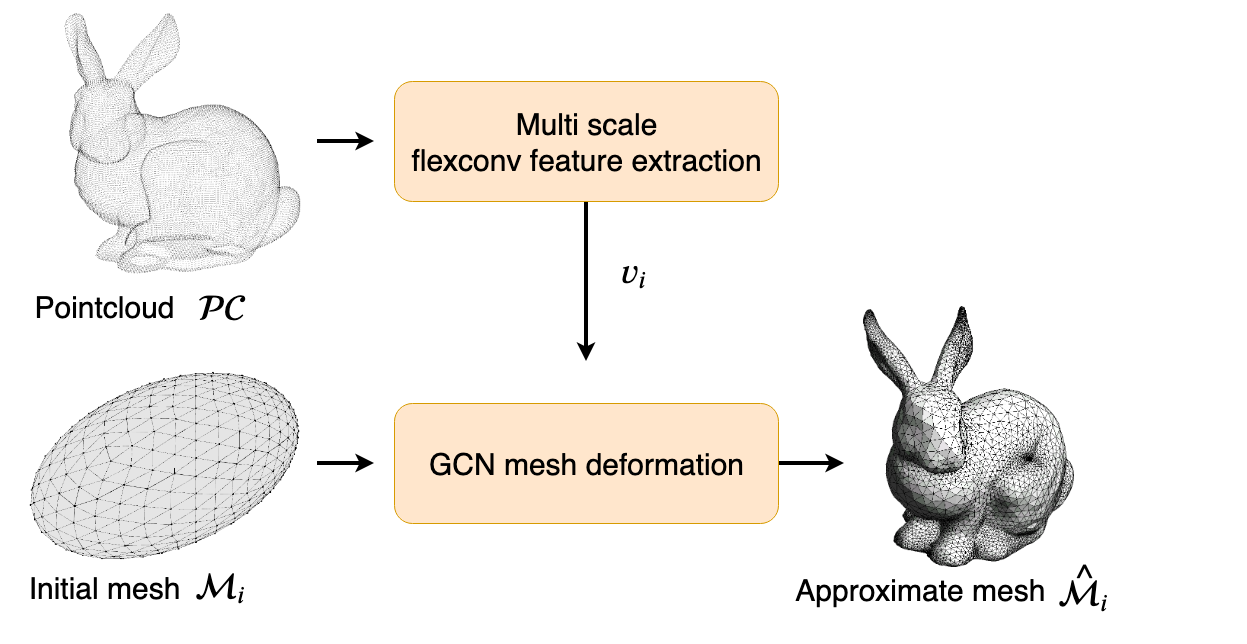
\includegraphics[width=14cm]{general_structure}
   \caption{General workflow of \emph{points2mesh} network. $\mathcal{N}_{recon}$ takes a pointcloud $\mathcal{PC}$ and an initial mesh $\mathcal{M}_i$
   as input, deforms $\mathcal{M}_i$ based on important features $v_i$ in $\mathcal{PC}$ to compute an approximate mesh $\hat{\mathcal{M}}$}
   \label{fig:generalconfig}
   \end{center}
 \end{figure}
 The general goal of the neural network $\mathcal{N}_{recon}$ is to provide an end-to-end solution for 
 explicit surface reconstruction given a collection of unstructured point cloud data ~(~$\mathcal{PC}$~) in three-dimensional 
 space with their normal orientation $\textbf{n}_{x_i}$. 

 With:
 \begin{align}
      \forall \textbf{x}_i \in \mathcal{PC} : 
      \textbf{x}_i =
      \begin{bmatrix}
            x \\
            y\\
            z
          \end{bmatrix} \in [-1,1]^3
   \end{align}

 Overall, the network structure is separated into two distinct parts,
  each with its specific purpose to fulfill. As seen in Figure \ref{fig:generalconfig}, the neural 
  network $\mathcal{N}_{recon}$ gets two different inputs, whereas each input is processed in a different part of the network.
 First, the input data $\mathcal{PC}$ is fed into the upper half of the network, called \emph{flexconv feature extraction}
  $\mathcal{N}_{flex}$ ~(~ See Figure \ref{fig:generalconfig} ~). In a multiscale convolutional operation,
   a collection of feature vectors $v_{x_n}$ is extracted, 
which is fed into the lower part of the network.

  The second part, as seen in the lower half of figure \ref{fig:generalconfig}, illustrates 
  a \emph{graph convolutional network} $\mathcal{N}_{gcn}$. Given an initial ellipsoid
  polygonal mesh $\mathcal{M}_{e}$, $\mathcal{N}_{gcn}$ deforms it, estimating $\hat{\mathcal{M}}$.
   Where $\hat{\mathcal{M}}$ is the best matching estimate for the ground truth mesh $\mathcal{M}_{gt}$ given $\mathcal{PC}$.
   The deformation process is assisted by supplying feature vectors $v_{x_n}$ from $\mathcal{N}_{flex}$, also adding more
    vertices to the initial ellipsoid $\mathcal{M}_{e}$ in three steps during the deformation process.
\subsection{Flexconv feature extraction}
\label{fconv}

\begin{figure}
   \begin{center}
   \includegraphics[width=14cm]{flexconv}
   \caption{$\mathcal{N}_{flex}$ with point cloud $\mathcal{PC}$ as input, computing features $v^j$ in three blocks of flexconv layers and a trailing flexpool layer  After each convolutional block, weighted random sampling reduces the number of samples of $\mathcal{PC}$ by a factor of four. Feature vectors $v^j$ are concatenated with their respective positions $x^j$ in a vector $\textbf{v}$.}
   \label{fig:flexconv}
   \end{center}
 \end{figure}

In traditional convolutional networks in context of computer graphics, the data at hand is often given as two dimensional images.
 In the case of three-dimensional processing, structured 3D grids are then a popular tool for natural processing 
 of such. However, since converting data from $\mathcal{PC}$ to a voxelized representation diminished its resolution, 
 it is now kept as its unstructured base form of point cloud data. 

As seen in the upper half of figure \ref{fig:flexconv}, $\mathcal{N}_{flex}$ processes $\mathcal{PC}$ to compute
 a collection of three feature vectors $v_{x_n}$ on a multiscale measure, working as follows.
 The network $\mathcal{N}_{flex}$ takes a vector of three-dimensional points $\textbf{x}_i \in \mathcal{PC}$ 
 of size $[3,1024]$ or $[3,8000]$ ~(~depending on the configuration ~), assigning each point its own 3D coordinates
  as his current feature $v_i$.
Then, it is separated into three consecutive parts, where each section $\mathcal{S}$ processes the point cloud vector $\textbf{x}_i$ and features $\textbf{v}_i$
 with two consecutive flexconv operators and a flexpool operator while expanding the dimension by a factor of $32$ in each section.
After convolving, the point cloud is sampled down by a factor of four each time by weighted reservoir sampling~(~wrs~)~. 
Following every convolution, the coordinates $\textbf{x}_i$ and their features $\textbf{v}_i$ are collected. 
This compiles the multiscale feature vector $v_i^s$, which consits of key points in $\mathcal{PC}$ needed for the deformation steps in the second part of the network.



\subsection{GCN mesh deformation}
   \label{gcnconv}
   \begin{figure}
      \begin{center}
      \includegraphics[width=14cm]{gcnpart}
      \caption{$\mathcal{N}_{gcn}$ with initial mesh $\mathcal{M}_i$ as input. Feature vector $\textbf{v}$ is
       projected onto the mesh $\mathcal{M}_i$ and deformed according to it. Then an unpooling layer increases
        the number of vertices in $\mathcal{M}_i$. Projecting $\textbf{v}$ onto the graph and deforming it afterward is repeated two more times.}
      \label{fig:gcn}
      \end{center}
   \end{figure}
   As for the second part of the network $\mathcal{N}_{recon}$, it consists 
   of a graph convolutional network $\mathcal{N}_{gcn}$, taking a basic polygonal 
   shape $\mathcal{M}_{i}$ as input, for example an ellipsoid form.
   The input mesh can directly be transformed into a graph structure, which the \emph{gcn}
   can process since each vertex in the mesh corresponds to a node in the graph.Its structure, i.e., 
   the number of vertices and edges, has to be known beforehand.
   Moreover, the same is true for the correspondence of edges in the mesh and edges in the graph. Thus, $\mathcal{M}_{i}=\mathcal{G}(V,E)$,
   with $V$ being the vertices in the graph, and $E$ the set of edges, connecting $V$.
   Furthermore, similarly to \ref{fconv}, the three-dimensional coordinates of each vertex in
   the initial mesh are utilized as feature vectors $f_i$ for $\mathcal{G}(V,E,f_i)$. Since $\mathcal{M}_{i}$ corresponds to $\mathcal{G}$, 
   in the following sections, the input graph $\mathcal{G}$ of $\mathcal{N}_{gcn}$ is still referenced as input mesh $\mathcal{M}_{i}$.
 
   $\mathcal{N}_{gcn}$ is separated into three parts, as seen in figure \ref{fig:gcn}.
   The primary process of one such segment consists of convolving on the graph for a set
   amount of iterations. Then, information from feature vectors $\textbf{v}_i$ from $\mathcal{N}_{flex}$ 
   to local feature vectors of the graph $f_i = [f_i,\textbf{v}_i]$ are appended by projecting them
   from the point cloud data onto the graph. Subsequently, the graph's vertices and edges are increased 
   with a specialized \emph{unpooling operation}. $\mathcal{N}_{gcn}$ repeats this process two more times 
   to compute $\hat{\mathcal{M}}$, approximating the underlying surface information for the input $\mathcal{PC}$.

   \label{gcnconv}
   \begin{figure}
      \begin{center}
      \includegraphics[width=10cm]{unpool}
      \caption{The \emph{unpooling} layer of $\mathcal{N}_{gcn}$ increases the
       number of vertices by introducing a new node between each neighboring node
        (~white~) in $\mathcal{M}_i$. A new node (~green~) is added precisely in 
        the middle of each old edge. Finally, the new nodes are connected, while also updating the neighborhood of the old nodes.}
      \label{fig:unpool}
      \end{center}
    \end{figure}

   The graph convolutional network is limited to a rigid structure of graphs on which it operates. 
   Thus, it is necessary to define it before starting to train the network. Theoretically, it is possible 
   to train the complete reconstruction with $\mathcal{N}_{recon}$ on an already highly detailed graph with 
   many edges and vertices. However, such a graph is harder to deform in a correct way to approximate $\hat{\mathcal{M}}$, 
   since it has many more trainable variables and thus may take much longer to converge, if at all. Hence, it would be easier to
   first deform an initial mesh with a low amount of detail, then increase its detail level over and over, deform anew, until it converges.
   Wang et al. \cite{wang2018pixel2mesh} describe an \emph{unpooling layer}, which enables $\mathcal{M}_i$ to gain more detail,
    every time it is applied to it (~$\mathcal{M}_0 \cdots \mathcal{M}_2$~). 
   This edge-based unpooling layer adds a new edge in the midpoint of each neighboring edge for the graph $\mathcal{G}$ as seen in 
   figure \ref{fig:unpool}. Subsequently, it connects the new ones, for that the amount of neighbors for each vertex stays the same. 
   Though, the structure of the resulting graphs has to be known as well. Otherwise stable training of $\mathcal{N}_{gcn}$ would not be possible. 
   $\mathcal{N}_{gcn}$ utilizes the layer twice, each time after deforming the current state of the graph and projecting $v_i$ 
   from the $\mathcal{PC}$ onto $\mathcal{M}_{i}$. 

   \begin{figure}
      \centering
      %\begin{subfigure}[a]{6cm}
      %   \includegraphics[width=6cm]{align}
      %   \caption{\todo{graph alignment, unbiased left, biased}}
      %\end{subfigure}
      %\begin{subfigure}[b]{6cm}
      %   \includegraphics[width=6cm]{no_align}
      %   \caption{Initial ellipsoid, placed in relation to input point cloud $\mathcal{PC}$.}
      %\end{subfigure}
      \includegraphics[width=6cm]{no_align}
      \includegraphics[width=6cm]{align}
      \caption{Initial ellipsoid in relation to input pointcloud $\mathcal{PC}$ before aligning on the left. After \emph{align graph} layer on the right.
      Thus, eliminating positional bias and letting the mesh shrink during deformation, rather than letting it grow.}
      \label{fig:align}
      %\end{center}
   \end{figure}

   
   Since the data in $\mathcal{PC}$, may not always be uniformly sampled ~(~See section \ref{dataset}~),
   it is essential to compensate for the positional bias of the $\mathcal{PC}$ in relation to $\mathcal{M}_{i}$ as seen in figure \ref{fig:align}. 
   $\mathcal{N}_{gcn}$ begins with a \textbf{graph alignment layer} , moving the arithmetic midpoint of the graph $\mathcal{M}_{i}$ 
   on top of the arithmetic midpoint of $\textbf{x}_i \in \mathcal{PC}$:
   \begin{align}
   \label{form:align}
   \forall \textbf{x}_{gcn} \in \mathcal{M}_i : \textbf{x}'_{gcn} = \textbf{x}_{gcn} + 
   (\frac{1}{|\mathcal{PC}|}\sum_{x_i \in \mathcal{PC}}x_i - \frac{1}{|\mathcal{M}_{i}|}\sum_{x_{gcn} \in \mathcal{M}_i}x_{gcn})
   \end{align}
   After repositioning the graph, it is rescaled to the value domain of $[-1,1]^3$, if it exceeds it.
   Besides, this facilitates learning a more generalized form for deforming the mesh, for that $\mathcal{N}_{gcn}$ can not rely on absolut but rather relative positioning of $\mathcal{M}_{i}$ during 
   convolution.

   \subsubsection*{Feature projection}
   \label{featureproj}
   \begin{figure}
      \begin{center}
      \includegraphics[width=5cm]{projection}
      \caption{\emph{graph projection} layer, assigning feature vectors $\textbf{v}^j$ to nodes in
       $\mathcal{M}_i$ based on the distance to their nearest neighbor in $\mathcal{PC}$.}
      \label{fig:proj}
      \end{center}
   \end{figure}

   Considering only \emph{convolutional operations}, \emph{graph alignment layer} and \emph{unpooling layer}
   of $\mathcal{N}_{gcn}$, a connection from $\mathcal{N}_{flex}$ has yet to be made. Ideally, a 
   correlation between $\mathcal{PC}$ and $\mathcal{M}_{i}$ is created. The goal of $\mathcal{N}_{gcn}$ is 
   to deform $\mathcal{M}_{i}$ based on learned feature vectors $\textbf{v}_i$ from $\mathcal{N}_{flex}$. 
   Mathematically by default, no direct correlation between these two exist. Thus, the 
   \emph{feature projection layer} is proposed. It assigns for each vertex in $\mathcal{M}_i$,
   features from $\mathcal{N}_{flex}$ based on the distance from $\mathcal{M}_{i}$ to their $k$-nearest 
   neighbors in $\mathcal{PC}$. 

   As seen in blue in figure \ref{fig:proj}, every point in $\mathcal{PC}$ resides in the same coordinate
   system as vertices $p_j \in \mathcal{M}(V,E)$ ~(~ Illustrated as green points with their connecting vertices in black ~).
   For each vertex $p_j$, the \emph{feature projection layer} computes the $k$-nearest neighbors in $\mathcal{PC}$ 
   ~(~Here $k=6$ ~). Higher values for $k$ compensate for unstable performance of nearest neighbor search, 
   while lower values speed up excecution and thus training time.
   Features $[\textbf{v}_n^s,\cdots,\textbf{v}_{n+k}^s]$ of points $[\textbf{x}_{n}^s,\cdots,\textbf{x}_{n+k}^s]$ are scaled by 
   the distances $d_i = |\textbf{x}_i  - p_j|$.
   The final feature vector $f_i$ assigned to $p_i$ is calculated like the following:
   \begin{align}
      \forall p_j \in \mathcal{M}_{i} : f_i^s &= \frac{1}{k}\sum_{\forall x_i^s \in knn(p_j),s\in \mathcal{S}} \frac{v_i^s}{1 + |x_i^s-p_j|^2}
   \end{align}
   Where $v_i$ is the respective feature vector stored at point $\textbf{x}_i^s$. This is repeated for each scaling $s$ in $\mathcal{S}$ of 
   $\mathcal{N}_{flex}$ where a feature vector is propagated out of the subnetwork ~(~ See figure \ref{fig:flexconv}~).

\subsection{Loss functions}
\label{lossfuncs}s
   The losses are defined based on the network of Wang et al. \cite{wang2018pixel2mesh}, 
   and adapted accordingly to work with point cloud based input data. Given $\textbf{x}_i$ 
   and normal orientation $\textbf{n}_i$, an objective function $\mathcal{F}$ is defined as 
   follows to help generate good-looking results.

   A symmetrical \emph{chamfer distance loss} $l_{ch}$ tries to ensure that vertices of $\mathcal{M}_{i}$ 
   are located close to other points $\textbf{x}_i$ in ground truth data $\mathcal{PC}$. It sums
   up for each vertex $p_j\in \mathcal{M}_i$ the distance to its nearest neighbor in $\mathcal{PC}$
   and for each point $\textbf{x}_i\in \mathcal{PC}$ the distance to its nearest neighbor in
   $\mathcal{M}_i$. Though, it is scaled by sizes of $|\textbf{x}_i|$ relative to $|p_j|$, depending on how often 
   $\mathcal{M}_i$ already has been unpooled (~See Appendix \ref{sec:appendix} for their formula~).

   Furthermore, Wang et al. propose an edge length loss $l_{edge}$ in $\mathcal{F}$ , reducing the overall mean of lengths of the edges.
   And scaling it up by a predetermined constant value of $300$, as seen in formula \ref{form:edge}. 
   Only considering $l_{ch}$ and $l_{edge}$ ignores the orientation of neighboring faces.
   Wang et al.'s $l_{cos}$ term guides $\mathcal{F}$ to orientate neighboring edges towards the 
   same direction since most real meshes have smooth surfaces. This approximating term is illustrated in formula \ref{form:cos}.
   Additionally, since $l_{ch},l_{edge},l_{cos}$ may still lead to optimizations which gravitate towards local minima, they introduce 
   a laplacian regularizer $l_{lap}$ which avoids self intersecting meshes and moving single vertices too freely during
    the deformation process (~See Appendix \ref{sec:appendix} for their formula~).
   \begin{align}
      \label{form:edge}
      l_{edge} &= \frac{300}{|E|}\sum_{e\in E}||e||^2\\
      \label{form:cos}
      l_{cos} &= \frac{1}{2|E|}\sum_{e\in E}normal(e) \cdot e
   \end{align}


   In most extreme cases, it is possible for different, not neighboring vertices to land on top on each other, or close to each other 
   with distances $< \epsilon$. Since this case is not covered by avoiding selfintersections with the laplacian regularizer, a 
   \emph{collapse loss} $l_{col}$ is included in $\mathcal{F}$, defined as:
   \begin{align}
      l_{col} &= \frac{1}{|\mathcal{M}_{i}|}\sum_{ nn(p_j)-p_j > \epsilon,\forall p_j \in \mathcal{M}_{i}} 1
   \end{align}

   $\mathcal{N}_{recon}$ optimizes against the objective function $\mathcal{F}=l_{ch}+l_{col}+l_{cos}+l_{edge}$
    to obtain an approximate mesh $\hat{\mathcal{M}}$ which characterizes $\mathcal{PC}$.

\subsection{Network configurations $\mathcal{C}$}
\label{configurations}
Finding suitable hyperparameters and an appropriate network structure 
is no easy task. Tuning hyperparameters in small increments, removing or including 
more layers in either $\mathcal{N}_{recon}$ or $\mathcal{N}_{flex}$ may change results drastically.
 Therefore, some configurations have advantages over other 
configuration, while still having disadvantages in other aspects.
Thus, several configurations have been carved out and are specified 
in detail later evaluation. This section illustrates how the configurations deviate from the general
 network structure presented in section \ref{generalsystem} through \ref{gcnconv}.
Though, every configuration uses an ellipsoid triangle/quad mesh $\mathcal{M}_{i}$ with $156$ vertices for the deformation process of $\mathcal{N}_{gcn}$.
Consecutive \emph{unpooling} operations increase the count to $618$, and finally to $2466$ vertices.

\textbf{$\mathcal{C}_1$: Baseconfiguration}
\begin{figure}
   \begin{center}
   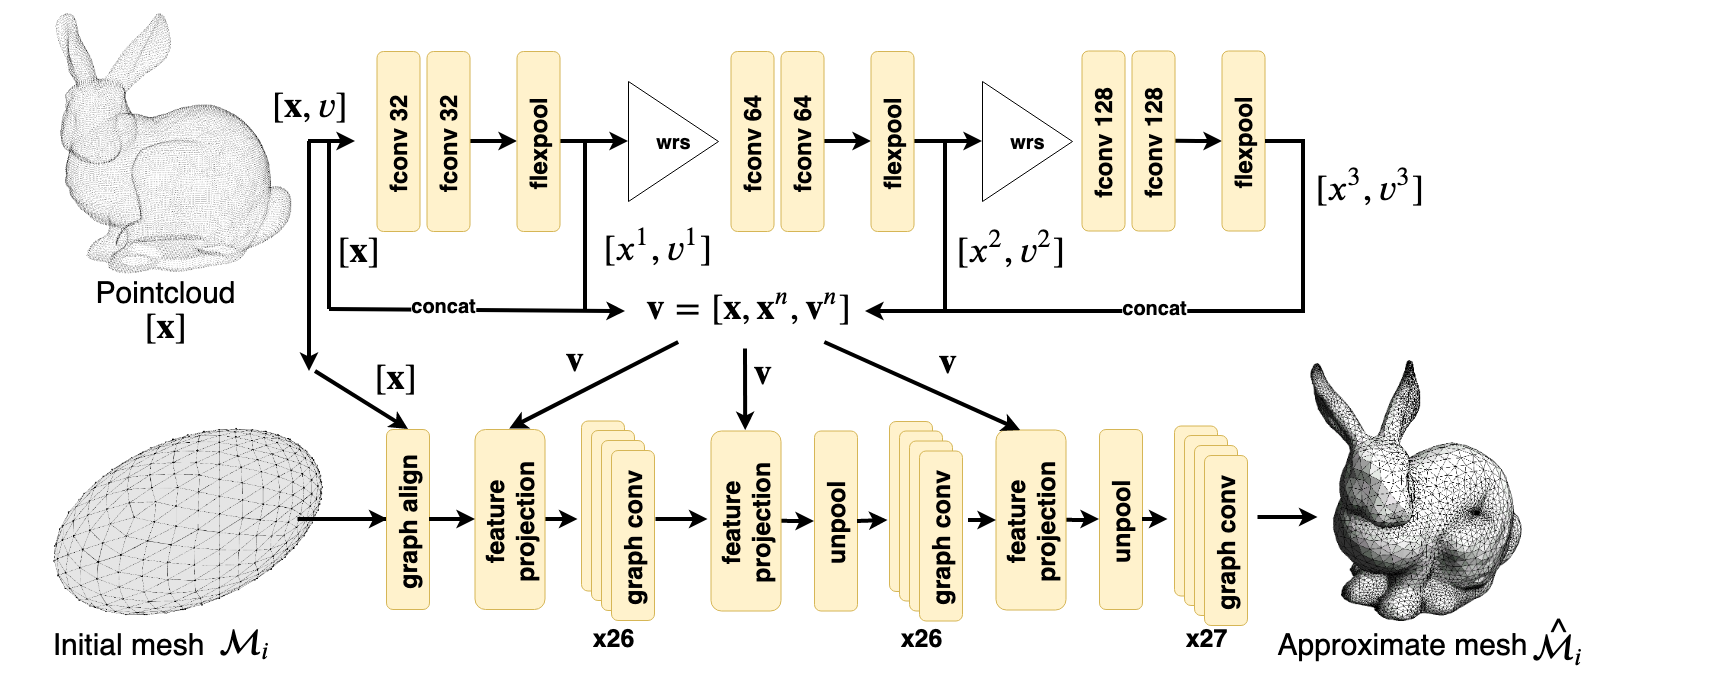
\includegraphics[width=14cm]{c1}
   \caption{Baseconfiguration $\mathcal{C}_1$ of $\mathcal{N}_{recon}$ showing flex conv feature extraction $\mathcal{N}_{flex}$ in the upper half, and
   graph deformation network $\mathcal{N}_{gcn}$ in the lower part. The complete network $\mathcal{N}_{recon}$ takes a point cloud and an initial mesh as input, 
   approximating the underlying surface information of the point cloud with $\hat{\mathcal{M}_i}$ after deforming the mesh, based on features learned in the point cloud}
    \label{fig:c1}
   \end{center}
\end{figure}
Configuration $\mathcal{C}_1$, as described in this chapter and seen in figure \ref{fig:c1},
 illustrates the base structure of $\mathcal{N}_{recon}$.
It is trained on an input $\mathcal{PC}$ with $1024$ as well as $800$ samples and increases
 the detail of $\mathcal{M}_{i}$ twice. 

\textbf{$\mathcal{C}_2$: High detailed baseconfiguration}
\begin{figure}
   \begin{center}
   \includegraphics[width=14cm]{c2}
   \caption{Configuration $\mathcal{C}_2$ of $\mathcal{N}_{recon}$, showing its difference in $\mathcal{N}_{gcn}$ to configuration $\mathcal{C}_1$.
   $\mathcal{C}_2$ introduces an extra \emph{projection}, \emph{unpooling} layer and a \emph{graph convolution} block. Thus, allowing for a higher detailed approximate mesh $\hat{\mathcal{M}}$ }
   \label{fig:c2}
   \end{center}
\end{figure}
Configuration $\mathcal{C}_2$ corresponds to $\mathcal{C}_1$ almost identically, 
with the exception of increasing the count of \emph{unpooling layer} from two to three, thus increasing
 the number of vertices to 10626. As seen in figure \ref{fig:c2} marked as green layer components, $\mathcal{N}_{gcn}$
  is expanded by appending another \emph{projection} and  \emph{unpooling} layer, as well
   as a \emph{convolution} block at the end. Similarly $\mathcal{C}_2$ is trained with $1024$ as well as $800$ samples
   in $\mathcal{PC}$.

\textbf{$\mathcal{C}_3$: Biased neighbor features}

Configuration $\mathcal{C}_3$, similarly configured like $\mathcal{C}_1$, but with a difference in the implementation of the \emph{projection layer}.
Instead of only projecting feature vectors $v_i$ of $\mathcal{PC}$ onto the mesh, it also adds the mean vector $\textbf{x}_i$ 
to the final feature vector $f_i^s$ for $\mathcal{M}_i$.
 \begin{align}
      \forall p_j \in \mathcal{M}_{i} : y_i^s &= \frac{1}{k}\sum_{\forall x_i^s \in knn(p_j),s\in \mathcal{S}} \frac{x_i^s}{1 + |x_i^s-p_j|^2}
   \end{align}
Thus, $\mathcal{N}_{gcn}$ utilizes the following feature vector $f_i$ after projecting in each detail step of the mesh $\mathcal{M}_i$:
\[f_i = [f_i, y_i^1, v_i^1, y_i^2, v_i^2,y_i^3, v_i^3,] \]
Additionally, as a variation of $\mathcal{C}_3$, the first layer of $\mathcal{N}_{gcn}$, the \emph{graph alignment layer} is omitted and 
thus defining configuration $\mathcal{C}'_3$. Removing the layer introduces a positional bias of the initial shape $\mathcal{M}_i$ into the network, but
leads to interesting reconstructions worthy of evaluating in more detail.

\textbf{$\mathcal{C}_4$: Compact GCN with simple projection}
\begin{figure}
   \begin{center}
   \includegraphics[width=14cm]{c4}
   \caption{Showing only $\mathcal{N}_{gcn}$ of $\mathcal{N}_{recon}$ with $\mathcal{N}_{flex}$ being the same
    as in configuration $\mathcal{C}_{1-3}$. In contrast to $\mathcal{C}_1$, Configuration $\mathcal{C}_4$ reduces 
    the number of used layers for deforming the mesh in $\mathcal{N}_{gcn}$.}
   \label{fig:c4}
   \end{center}
\end{figure}
Finally, based on configuration $\mathcal{C}_1$, configuration $\mathcal{C}_4$ reduces the amount of convolutional layers in $\mathcal{N}_{gcn}$ as seen in figure \ref{fig:c4}.
Furthermore, the distance based falloff $\frac{1}{1+d}$ in the \emph{projection layer} is excluded, 
while also computing only one nearest neighbor, $k=1$ in that particular layer. 

\section{Dataset}
\label{dataset}
   Finding and designing a suitable dataset $\mathcal{D}$
   to train the network on is just as crucial as designing its structure. 
   Such a suitable dataset is \emph{ModelNet}, offering 40 different object 
   categories and thousands of fully meshed objects. By default, it does not offer a
   point cloud representation, as required by $\mathcal{N}_{recon}$. Qi et al.
   \cite{qi2017pointnetplusplus} propose a transformation of the classical \emph{ModelNet40}
   dataset to a point cloud based one which can be utilized by $\mathcal{N}_{recon}$.

   This section describes their way of transforming the dataset, on which categories
   $\mathcal{N}_{recon}$ is trained on, and an additional data augmentation step to
   enhance the dataset.

\subsection{Dataset generation}
\todo{hier?}
\subsection{Utilized object categories}
\label{sec:categ}
\todo{Bilder fuer object categories or interesting features}
Even though \emph{ModelNet40}, and therefore the transformed point cloud dataset by Qi et al. offers, as the name suggests,
40 different object categories, only a subset of them is chosen for training purposes of $\mathcal{N}_{recon}$. 
The subset of $\mathcal{D}_{m40}$ is defined as $\mathcal{D}_{big}=[airplane,bed,bottle,bowl,chair,guitar,toilet]$
It is chosen based on the goal of learning a generalized deformation operation by showing preferably vastly different object categories
to the network, all with interesting object features, which $\mathcal{N}_{recon}$ should learn.

Point cloud data used for inference is not always sampled perfectly on the surface of an object. Random noise on these coordinates is common occurance.
For that reason, to aid $\mathcal{N}_{recon}$ learning a more generalized reconstruction, each of the dataset categories are
 augmented with random noise added to each vertex in the point cloud by a factor $q_{noise}$.

 Interesting features for reconstruction include:
 \begin{itemize}
   \item long appendages (~leg of a chair, airplane propellor~)
   \item thin appendages (~airplane wings~)
   \item hard edges (~toilet flushing cistern~)
   \item uniform curvatures (~bowl~)
   \item objects of \emph{genus} $>0$ (~some chairs/airplanes,guitars~)
 \end{itemize}


\chapter{Results}
\label{chap:results}

    By the nature of the defined configurations $\mathcal{C}_i$, the neural network
    \emph{points2mesh} has several reconstructions for each input point cloud $\mathcal{PC}$.
    Since it is not easy to estimate the quality of reconstructed meshes only based on numerical
    values, it is vital to assess their visual quality, tough highly subjective.
    Therefore, in this chapter, a wide range of reconstructed objects of various categories $\mathcal{C}_i$
    are presented and displayed next to their input point cloud $\mathcal{PC}$ and their ground 
    truth mesh. Some interesting features of reconstructions are pointed out, and presented with reconstructions of comparable
    reconstruction methods, as well as the alternative approach to train the network as outline in \ref{trainings}.
    
\section{Compared methods}

Restoring polygonal meshes directly from point cloud data is a new domain of geometry reconstruction, 
which yet has to be explored deeply. Apart from \emph{points2mesh}, no other methods relying on neural 
networks and deep learning techniques have yet been proposed for this kind of mode of data transformation.
For this reason, \emph{points2mesh} has to compete against techniques from traditional approaches like
\emph{ball-pivoting algorithm} \cite{817351}(~BPA~) and \emph{instant field meshes} \cite{Jakob2015Instant} (~IFM~). Furthermore, by adding
an intermediate step of voxelization of $\mathcal{PC}$, this work also can be compared against 
\emph{deep marching cubes} \cite{Liao2018CVPR} (~DMC~), which transforms voxelized data into meshes based on deep learning approaches and the classical
marching cubes algorithm.

\section{Result visualization}
% 1024Figure
  \ref{fig:1} shows the reconstruction from a point cloud sample size of 1024 from the \emph{category}
  \emph{airplane}. \ref{fig:1a} shows the ground truth mesh, and \ref{fig:1d} its sampled point cloud. Figures
  \ref{fig:1b}, \ref{fig:1c}, \ref{fig:1e}, \ref{fig:1f} show the reconstruction from $\mathcal{N}_{recon}$ with 
  configurations $\mathcal{C}_1$ through $\mathcal{C}_4$.

\begin{figure}[htbp]
  \centering
  \subfloat[Ground truth mesh.\label{fig:1a}]{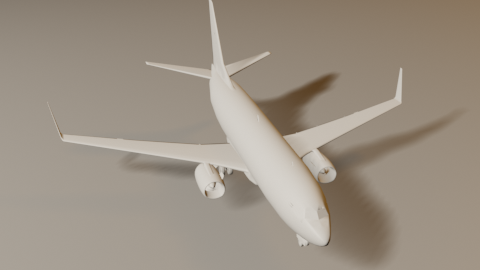
\includegraphics[width=0.32\textwidth]{gt_airplane_1.png}}
  \subfloat[Configuration $\mathcal{C}_1$.\label{fig:1b}]{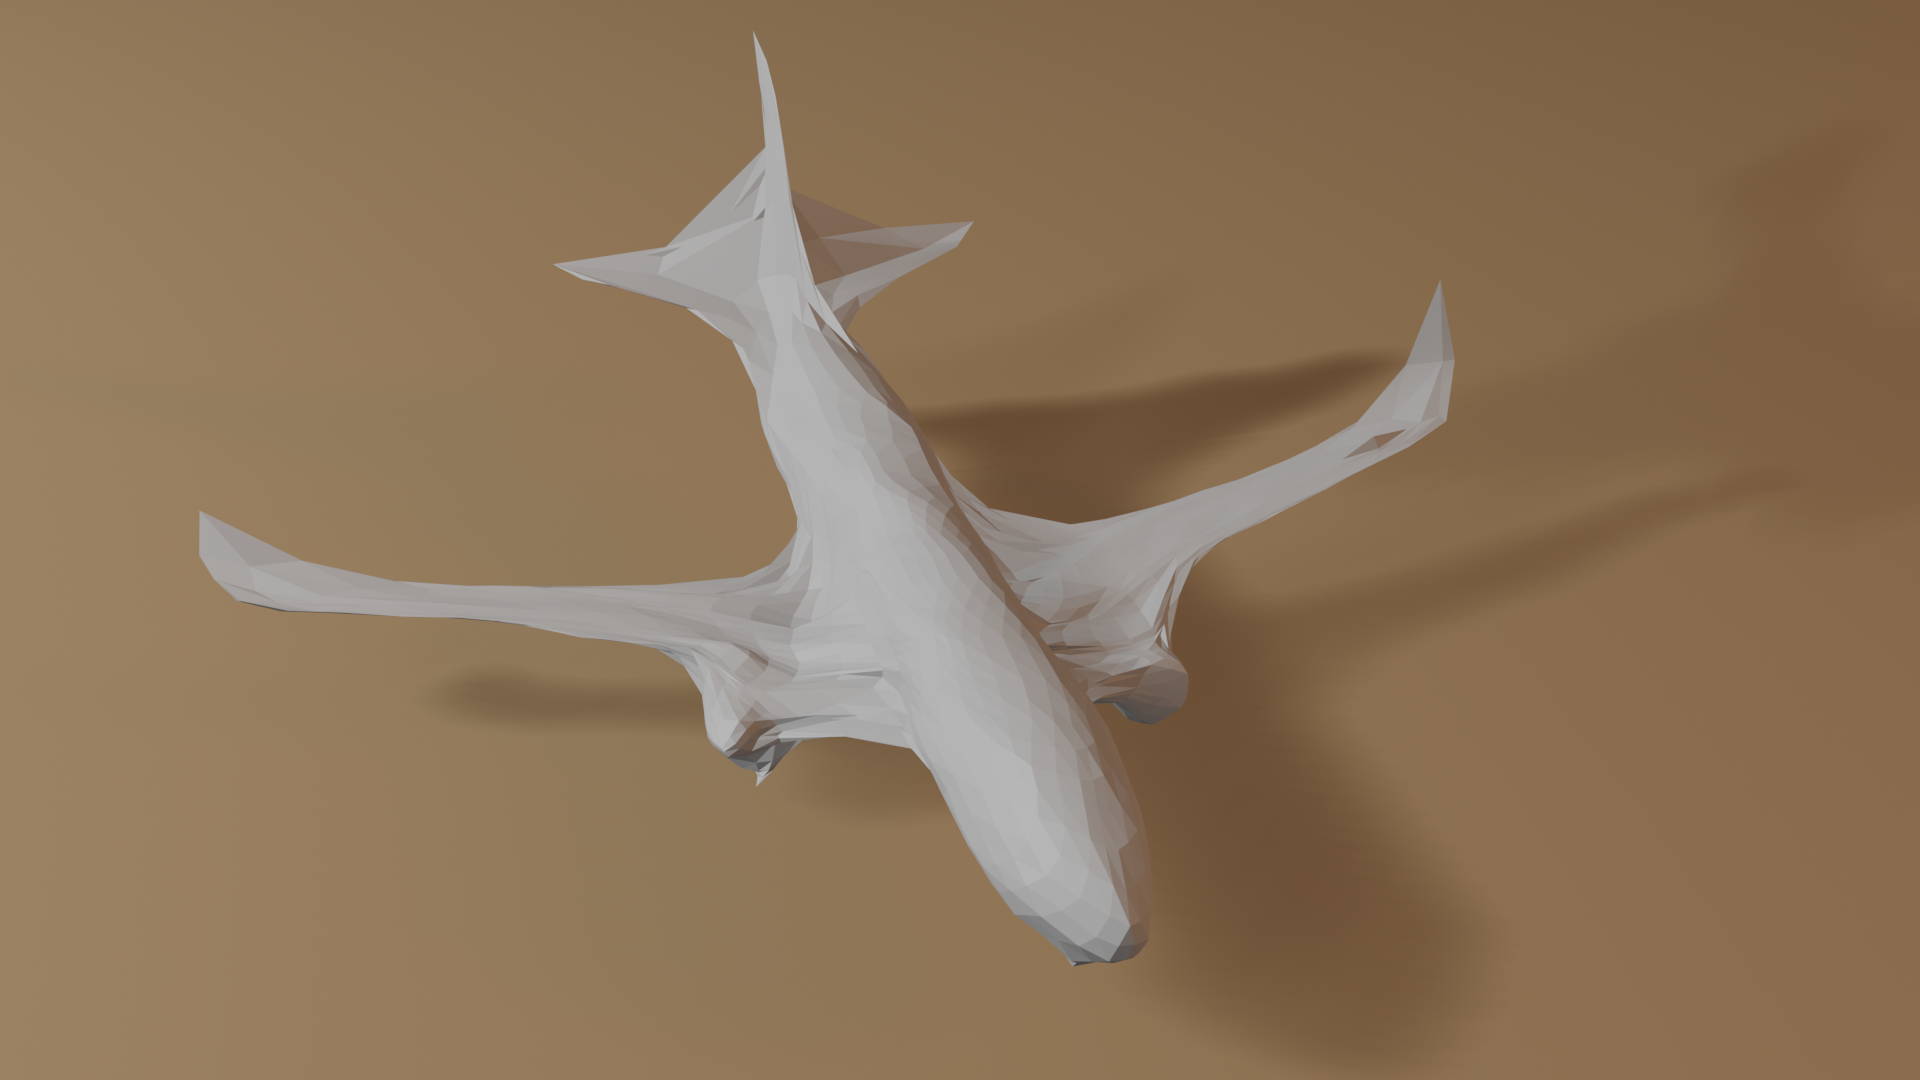
\includegraphics[width=0.32\textwidth]{c1_1024_airplane_1.png}}
  \subfloat[Configuration $\mathcal{C}_2$.\label{fig:1c}]{\includegraphics[width=0.32\textwidth]{c2_1024_airplane_1.png}}\\
  \subfloat[Sampled point cloud from ground truth mesh.\label{fig:1d}]{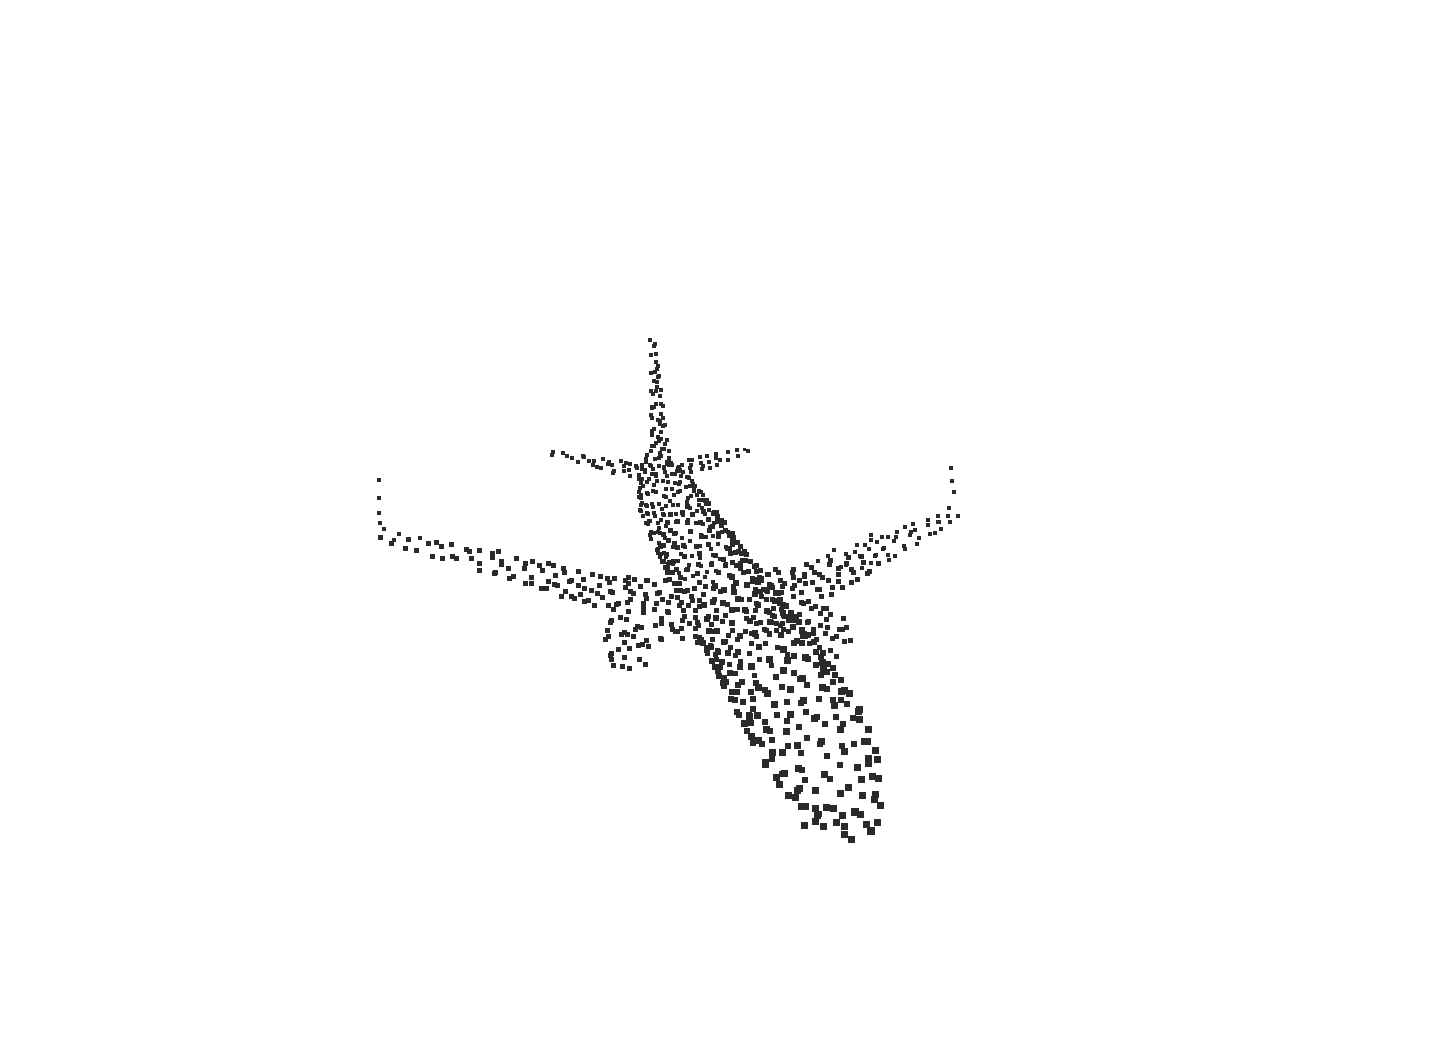
\includegraphics[width=0.32\textwidth]{airplane_1_pc.png}}
  \subfloat[Configuration $\mathcal{C}_3$.\label{fig:1e}]{\includegraphics[width=0.32\textwidth]{c3_1024_airplane_1.png}}
  \subfloat[Configuration $\mathcal{C}_4$.\label{fig:1f}]{\includegraphics[width=0.32\textwidth]{c4_1024_airplane_1.png}}\\
  \subfloat[Reconstrucion with \emph{BPA}.\label{fig:1g}]{\includegraphics[width=0.32\textwidth]{airplane_bpa_1024.png}}
  \subfloat[Reconstruction with \emph{IFM}.\label{fig:1h}]{\includegraphics[width=0.32\textwidth]{ifm_1024_airplane_1.png}}
  \subfloat[Reconstruction with \emph{DMC}.\label{fig:1i}]{\includegraphics[width=0.32\textwidth]{dmc_airplane.png}}
  \caption{Reconstruction of an airplane from point cloud with 1024 samples.} \label{fig:1}
\end{figure}

\begin{figure}[htbp]
  \centering
  \subfloat[Ground truth mesh.\label{fig:2a}]{\includegraphics[width=0.32\textwidth]{gt_chair_1.png}}
  \subfloat[Configuration $\mathcal{C}_1$.\label{fig:2b}]{\includegraphics[width=0.32\textwidth]{c1_1024_chair_1.png}}
  \subfloat[Configuration $\mathcal{C}_2$.\label{fig:2c}]{\includegraphics[width=0.32\textwidth]{c2_1024_chair_1.png}}\\
  \subfloat[Configuration $\mathcal{C}_3$.\label{fig:2d}]{\includegraphics[width=0.32\textwidth]{c3_1024_chair_1.png}}
  \subfloat[Configuration $\mathcal{C}_4$.\label{fig:2epro}]{\includegraphics[width=0.32\textwidth]{c4_1024_chair_1.png}}
  \caption{Reconstruction of a chair from point cloud with 1024 samples.} \label{fig:2}
\end{figure}

\begin{figure}[htbp]
  \centering
  \subfloat[Ground truth mesh.\label{fig:3a}]{\includegraphics[width=0.32\textwidth]{gt_guitar_1.png}}
  \subfloat[Configuration $\mathcal{C}_1$.\label{fig:3b}]{\includegraphics[width=0.32\textwidth]{c1_1024_guitar_1.png}}
  \subfloat[Configuration $\mathcal{C}_2$.\label{fig:3c}]{\includegraphics[width=0.32\textwidth]{c2_1024_guitar_1.png}}\\
  \subfloat[Sampled point cloud from ground truth mesh.\label{fig:3d}]{\includegraphics[width=0.32\textwidth]{guitar_pc00.png}}
  \subfloat[Configuration $\mathcal{C}_3$.\label{fig:3e}]{\includegraphics[width=0.32\textwidth]{c3_1024_guitar_1.png}}
  \subfloat[Configuration $\mathcal{C}_4$.\label{fig:3f}]{\includegraphics[width=0.32\textwidth]{c4_1024_guitar_1.png}}\\
  \subfloat[\emph{IFM} guitar reconstruction.\label{fig:3g}]{\includegraphics[width=0.32\textwidth]{ifm_1024_guitar_1.png}}
  \subfloat[\emph{DMC} guitar reconstruction.\label{fig:3h}]{\includegraphics[width=0.32\textwidth]{dmc_guitar.png}}
  \caption{Reconstruction of a guitar from point cloud with 1024 samples.} \label{fig:3}
\end{figure}
\begin{figure}[htbp]
  \centering
  \subfloat[Ground truth mesh.\label{fig:4a}]{\includegraphics[width=0.32\textwidth]{gt_bowl_1.png}}
  \subfloat[Configuration $\mathcal{C}_1$.\label{fig:4b}]{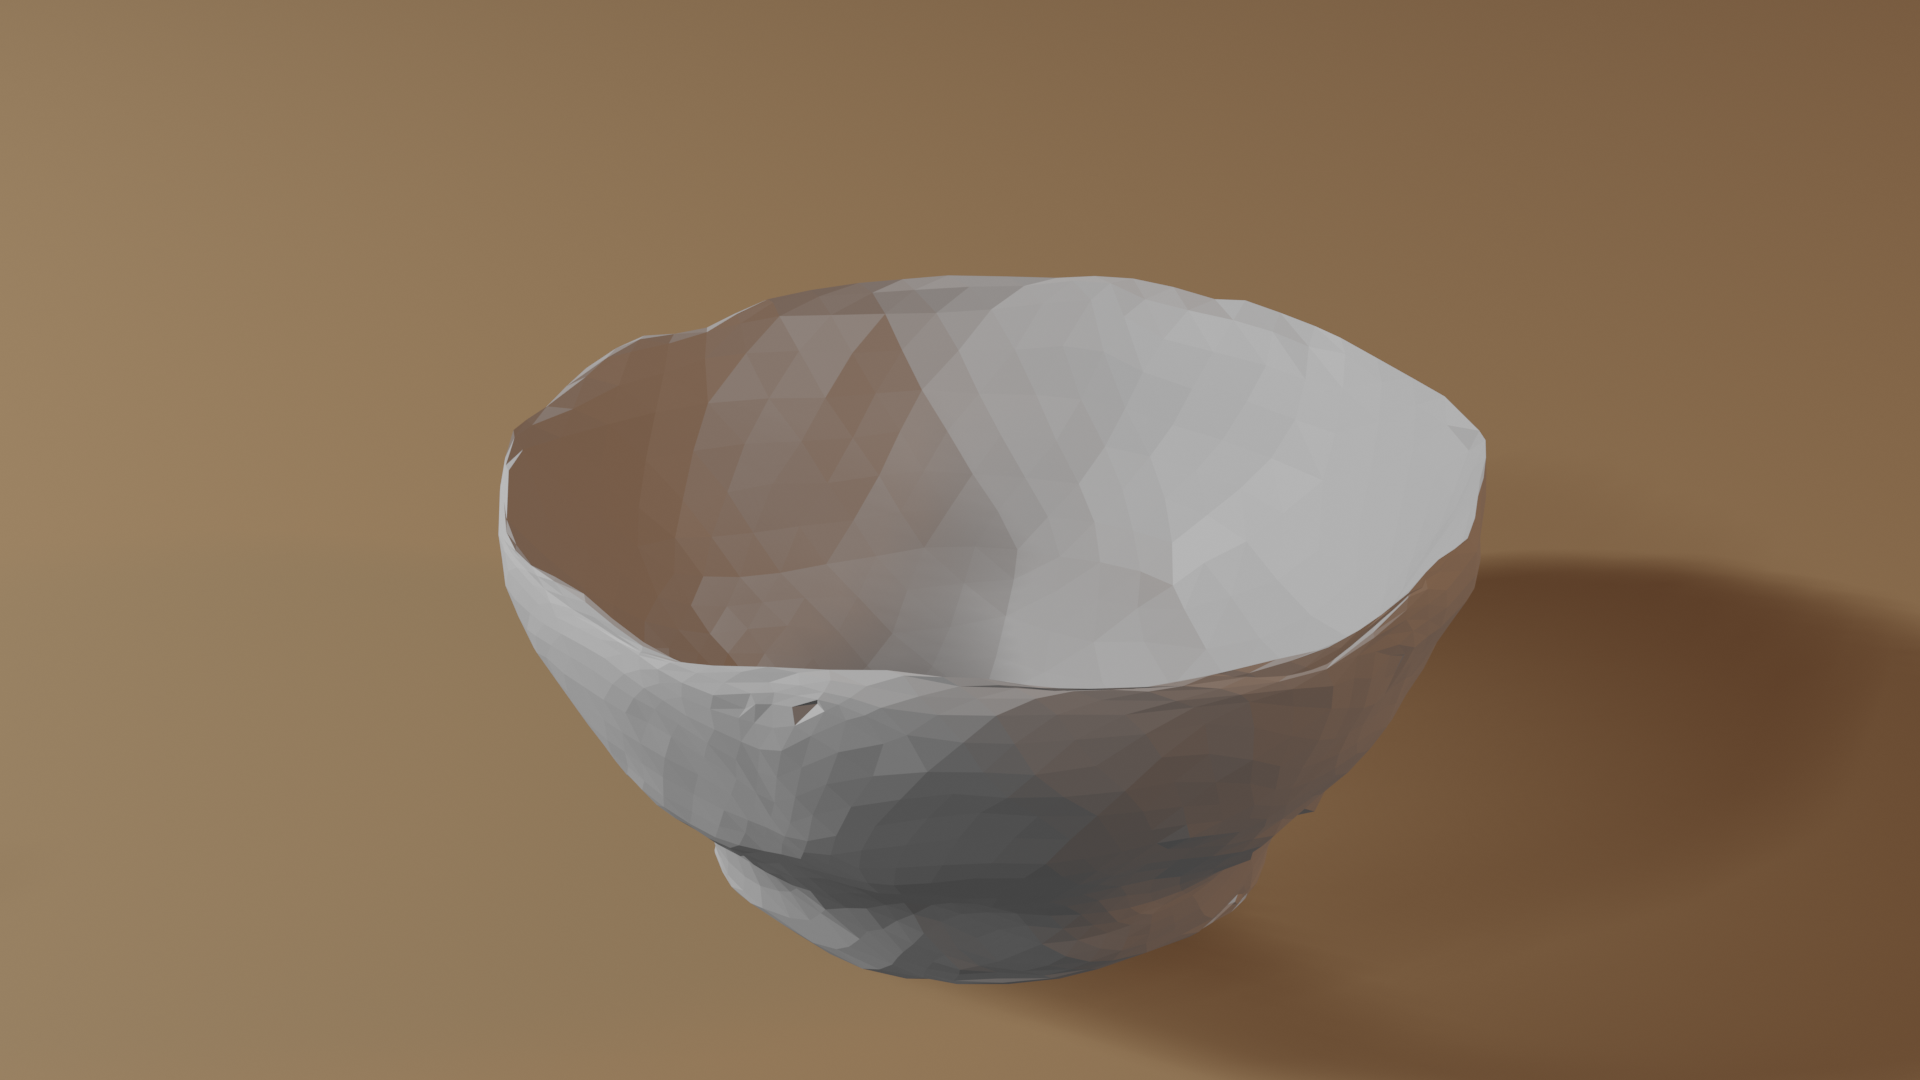
\includegraphics[width=0.32\textwidth]{c1_1024_bowl_1.png}}
  \subfloat[Configuration $\mathcal{C}_2$.\label{fig:4c}]{\includegraphics[width=0.32\textwidth]{c2_1024_bowl_1.png}}\\
  \subfloat[Reconstruction with \emph{DMC}\label{fig:4d}]{\includegraphics[width=0.32\textwidth]{dmc_bowl.png}}
  \subfloat[Configuration $\mathcal{C}_3$.\label{fig:4e}]{\includegraphics[width=0.32\textwidth]{c3_1024_bowl_1.png}}
  \subfloat[Configuration $\mathcal{C}_4$.\label{fig:4f}]{\includegraphics[width=0.32\textwidth]{c4_1024_bowl_1.png}}
  \caption{Reconstruction of a bowl from point cloud with 1024 samples.} \label{fig:4}
\end{figure}

  The last row depicts reconstructions with \emph{BPA}, \emph{IFM}, and \emph{DMC}. While the reconstruction with configuration 
  $\mathcal{C}_1$ represents the most interesting features of the airplane, especially the small winglets, it still has some errors. 
  One of the errors is at the rear of the plane with an edge dangling in the air, spanning over it. The same error happens with configuration
  $\mathcal{C}_3$ and $\mathcal{C}_4$ too. Configuration $\mathcal{C}_2$ seems to represent the airplane's features the best, though the least
  smooth of all reconstructions. As seen in figures \ref{fig:1f} and \ref{fig:2c}, configuration $\mathcal{C}_2$ is generally depicting the ground
    truth mesh in a good way, though not smooth.
  Considering other reconstruction methods, different problems, but also positives can be seen. \emph{BPA} reproduces smooth results as seen 
  in figure \ref{fig:1g}, while \emph{IFM} does not perform as well on low samples (~256 and 1024~) as seen in figure \ref{fig:1h}. Generally 
  \emph{DMC} does not perform good either as seen in figures \ref{fig:1i} and \ref{fig:3h}.

  Similarly, figure \ref{fig:2} through \ref{fig:5} show reconstructions with the same configurations $\mathcal{C}_i$ from $\mathcal{N}_{recon}$,
  but with an object from the categories \emph{chair}, \emph{guitar}, \emph{bowl}. These categories were included
  in the training set of $\mathcal{N}_{recon}$, though every reconstructed object sample originate from a test set, and thus have not be seen
  during the training stage.
  Similar behavior of the four network configurations, as described above, can be seen again, including the spanning of edges over empty space,
  like in figure \ref{fig:2d}, between the legs of the chair.
% 256
\begin{figure}[htbp]
  \centering
  \centering
  \subfloat[Ground truth mesh.\label{fig:5a}]{\includegraphics[width=0.5\textwidth]{gt_chair_256_1.png}}
  \subfloat[Ground truth mesh.\label{fig:5b}]{\includegraphics[width=0.5\textwidth]{gt_chair_7500.png}}\\
  \subfloat[Sampled point cloud from ground truth mesh.\label{fig:5b}]{\includegraphics[width=0.5\textwidth]{chair_256_pc06.png}}
  \subfloat[Sampled point cloud from ground truth mesh.\label{fig:5c}]{\includegraphics[width=0.5\textwidth]{chair_256_pc00.png}}\\
  \subfloat[Configuration $\mathcal{C}_1$.\label{fig:5d}]{\includegraphics[width=0.5\textwidth]{c1_256_chair_1.png}}
  \subfloat[Configuration $\mathcal{C}_2$.\label{fig:5e}]{\includegraphics[width=0.5\textwidth]{c1_256_chair_2.png}}\\
  \caption{Reconstruction of chairs from point cloud with 256 samples.} \label{fig:5}
\end{figure}
\begin{figure}[htbp]
  \centering
  \subfloat[Ground truth mesh.\label{fig:51a}]{\includegraphics[width=0.5\textwidth]{gt_car_1.png}}
  \subfloat[Sampled point cloud from ground truth mesh.\label{fig:51b}]{\includegraphics[width=0.5\textwidth]{car_pc05.png}}\\
  \subfloat[Configuration $\mathcal{C}_1$.\label{fig:51c}]{\includegraphics[width=0.5\textwidth]{c1_256_car_1.png}}
  \subfloat[Reconstruction of car with \emph{DMC},.\label{fig:51d}]{\includegraphics[width=0.5\textwidth]{dmc_car.png}}
  \caption{Reconstruction of a car from point cloud with 256 samples.} \label{fig:51}
\end{figure}
\begin{figure}[htbp]
  \centering
  \subfloat[Ground truth mesh.\label{fig:52a}]{\includegraphics[width=0.33\textwidth]{gt_256_toilet.png}}
  \subfloat[Configuration $\mathcal{C}_1$.\label{fig:52b}]{\includegraphics[width=0.33\textwidth]{c1_256_toilet.png}}
  \subfloat[Reconstruction with \emph{BPA}\label{fig:52c}]{\includegraphics[width=0.33\textwidth]{bpa_256_toilet.png}}
  \caption{Reconstruction of a toilet from point cloud with 256 samples.} \label{fig:52}
\end{figure}
  Figures \ref{fig:5} and \ref{fig:51} show reconstruction with a sample size of 256. Depicted are reconstructions with configurations
  $\mathcal{C}_1$ and $\mathcal{C}_2$ 
  and their corresponding ground truth mesh and sampled point cloud.
  While still able to reconstruct the general shape of the object, the spanning problem is still visible.
  Additionally, \emph{DMC} is not able to handle bigger empty spaces in the sparse cloud well enough to create a proper reconstruction,
  as seen in figure \ref{fig:51d}.


  \begin{figure}[htbp]
    \centering
    \subfloat[Ground truth mesh.\label{fig:6a}]{\includegraphics[width=0.4\textwidth]{gt_chair_7500.png}}
    \subfloat[Sampled point cloud from ground truth mesh.\label{fig:6b}]{\includegraphics[width=0.4\textwidth]{chair_pc00.png}}\\
    \subfloat[Configuration $\mathcal{C}_1$.\label{fig:6c}]{\includegraphics[width=0.4\textwidth]{c1_7500_chair_2.png}}
    \subfloat[Configuration $\mathcal{C}_4$.\label{fig:6d}]{\includegraphics[width=0.4\textwidth]{c4_7500_chair_2.png}}
    \caption{Reconstruction of a chair from point cloud with 7500 samples.} \label{fig:6}
  \end{figure}
  \begin{figure}[htbp]
    \centering
    \subfloat[Ground truth mesh.\label{fig:61a}]{\includegraphics[width=0.4\textwidth]{gt_airplane_7500.png}}
    \subfloat[Samples pointc loud from ground truth mesh.\label{fig:6d}]{\includegraphics[width=0.4\textwidth]{plane2_pc04.png}}\\
    \subfloat[Configuration $\mathcal{C}_1$.\label{fig:6e}]{\includegraphics[width=0.4\textwidth]{c4_7500_airplane_2.png}}
    \subfloat[Configuration $\mathcal{C}_4$.\label{fig:6f}]{\includegraphics[width=0.4\textwidth]{c1_7500_airplane_2.png}}
    \caption{Reconstruction of an airplane from point cloud with 7500 samples.} \label{fig:61}
  \end{figure}
  
  Figures \ref{fig:6} and \ref{fig:61} show reconstruction of a chair and an airplane from 7500 samples. Depicted are configurations 
  $\mathcal{C}_1$ and $\mathcal{C}_4$.


% 7500

%256-1024-7500
\begin{figure}[htbp]
  \centering
  \subfloat[Ground truth mesh.\label{fig:7a}]{\includegraphics[width=0.5\textwidth]{gt_airplane_7500.png}}
  \subfloat[$\mathcal{C}_1$ with sample size 256.\label{fig:7b}]{\includegraphics[width=0.5\textwidth]{c1_256_airplane_2.png}}\\
  \subfloat[$\mathcal{C}_1$ with sample size 1024.\label{fig:7c}]{\includegraphics[width=0.5\textwidth]{c1_1024_airplane_2.png}}
  \subfloat[$\mathcal{C}_1$ with sample size 7500.\label{fig:7d}]{\includegraphics[width=0.5\textwidth]{c4_7500_airplane_2.png}}\\
  \subfloat[\emph{BPA} with sample size 7500.\label{fig:7e}]{\includegraphics[width=0.5\textwidth]{airplane2_ifm_7500.png}}
  \subfloat[\emph{IFM} with sample size 7500.\label{fig:7f}]{\includegraphics[width=0.5\textwidth]{airplane2_bpa_7500.png}}
  \caption{Reconstruction of an airplane with different sample sizes, but the same configuration $\mathcal{C}_1$.} \label{fig:7}
\end{figure}

  For easier comparisons, figure \ref{fig:7} shows the reconstruction of the same airplane with configuration $\mathcal{C}_1$ but with
  different sample sizes, as well as reconstructions from \emph{BPA} and \emph{IFM} with the same sample size, showing their ostensible
  superiority with more samples.


  \begin{figure}[htbp]
    \centering
    \subfloat[Noisy airplane 1.\label{fig:81a}]{\includegraphics[width=0.5\textwidth]{c1_1024_noise_airplane_1.png}}
    \subfloat[Noisy airplane 2.\label{fig:81b}]{\includegraphics[width=0.5\textwidth]{c1_1024_noise_airplane_2.png}}\\
    \subfloat[Noisy airplane 3.\label{fig:81c}]{\includegraphics[width=0.5\textwidth]{c1_1024_noise_airplane_3.png}}
    \subfloat[Noisy airplane 4.\label{fig:81d}]{\includegraphics[width=0.5\textwidth]{c1_1024_noise_airplane_4.png}}
    \caption{Reconstruction of airplanes with $\mathcal{C}_1$ from noisy point cloud with noise factor of $0.01$. } \label{fig:81}
  \end{figure}
  Next, in figure \ref{fig:81}, reconstruction of airplanes and with configuration $\mathcal{C}_1$ can be seen. Each point in the point 
  cloud has random
  jitter noise between $-0.01$ and $0.01$ added on top of it.


% generalization
\begin{figure}[htbp]
  \centering
  \subfloat[Ground truth mesh.\label{fig:8a}]{\includegraphics[width=0.32\textwidth]{gt_person_1.png}}
  \subfloat[$\mathcal{C}_1$.\label{fig:8b}]{\includegraphics[width=0.32\textwidth]{c1_1024_person_1.png}}
  \subfloat[$\mathcal{C}_2$.\label{fig:8c}]{\includegraphics[width=0.32\textwidth]{c2_1024_person_1.png}}\\
  \subfloat[Sampled point cloud from ground truth mesh.\label{fig:8d}]{\includegraphics[width=0.32\textwidth]{person_pc00.png}}
  \subfloat[$\mathcal{C}_3$.\label{fig:8e}]{\includegraphics[width=0.32\textwidth]{c3_1024_person_1.png}}
  \subfloat[$\mathcal{C}_4$.\label{fig:8f}]{\includegraphics[width=0.32\textwidth]{c4_1024_person_1.png}}
  \caption{Reconstruction from point clouds of untrained category \emph{person}.} \label{fig:8}
\end{figure}
\begin{figure}[htbp]
  \centering
  \subfloat[$\mathcal{C}_1$.\label{fig:9a}]{\includegraphics[width=0.5\textwidth]{c1_1024_bathtub_1.png}}
  \subfloat[$\mathcal{C}_2$.\label{fig:9b}]{\includegraphics[width=0.5\textwidth]{c2_1024_bathtub_1.png}}\\
  \subfloat[$\mathcal{C}_3$.\label{fig:9c}]{\includegraphics[width=0.5\textwidth]{c3_1024_bathtub_1.png}}
  \subfloat[$\mathcal{C}_4$.\label{fig:9d}]{\includegraphics[width=0.5\textwidth]{c4_1024_bathtub_1.png}}
  \caption{Reconstruction from point clouds of untrained category \emph{bathutb}.} \label{fig:9}
\end{figure}
\begin{figure}[htbp]
  \centering
  \subfloat[Input point cloud of stone goblet.\label{fig:ca}]{\includegraphics[width=0.32\textwidth]{bappc.png}}
  \subfloat[Texturized reconstruction with photogammetry.\label{fig:cb}]{\includegraphics[width=0.32\textwidth]{bapgt.png}}
  \subfloat[Reconstruction with $\mathcal{C}_2$ with 1024 samples.\label{fig:cc}]{\includegraphics[width=0.32\textwidth]{bap.png}}\\
  \subfloat[Input point cloud toy propellor plane.\label{fig:da}]{\includegraphics[width=0.32\textwidth]{prpc.png}}
  \subfloat[Texturized reconstruction with photogammetry.\label{fig:db}]{\includegraphics[width=0.32\textwidth]{prgt.png}}
  \subfloat[Reconstruction with $\mathcal{C}_2$ with 1024 samples.\label{fig:dc}]{\includegraphics[width=0.32\textwidth]{prhigh.png}}
  \caption{Reconstruction from point cloud of objects unrelated to ModelNet40. Top row depicts a 3D scanned goblet. Bottom row depicts a 3D scanned toyairplane.
  Both objects offered scanned point cloud which has been downsampled to fit for \emph{points2mesh}} \label{fig:generalgeneral}
\end{figure}
\begin{figure}[htbp]
  \centering
  \subfloat[Point cloud of stanford bunny before downsampling.\label{fig:ba}]{\includegraphics[width=0.32\textwidth]{bunny_pc.png}}
  \subfloat[Reconstruction with $\mathcal{C}_1$ with 1024 samples.\label{fig:bb}]{\includegraphics[width=0.32\textwidth]{bunny.png}}
  \subfloat[Reconstruction with $\mathcal{C}_2$ with 1024 samples.\label{fig:bc}]{\includegraphics[width=0.32\textwidth]{bunnyhigh.png}}
  \caption{Reconstruction from point cloud of an object unrelated to ModelNet40.} \label{fig:bunny}
\end{figure}
  Figure \ref{fig:8} and figure \ref{fig:9} show the reconstruction of a person and a bathtub, based on point cloud samples 
  which $\mathcal{N}_{recon}$ has not been trained with. Additionally, figures \ref{fig:generalgeneral} and \ref{fig:bunny} show
  reconstruction from point clouds unrelated to the dataset ModelNet40. Figure \ref{fig:cb} depicts a 3D scanned goblet, figure \ref{fig:db} a scanned
  toy plane and figure \ref{fig:ba} a point cloud of the stanford bunny. Nevertheless, \emph{points2mesh} is able to reconstruct these objects. Though, the bunny much
  better than either the toy plane or the goblet.
\begin{figure}[htbp]
 \centering
 \subfloat[Reconstruction with 256 samples\label{fig:12a}]{\includegraphics[width=0.33\textwidth]{c1_opt_256_airplane2.png}}
  \subfloat[Reconstruction with 1024 samples\label{fig:12b}]{\includegraphics[width=0.33\textwidth]{c1_opt_1024_airplane2.png}}
  \subfloat[Reconstruction with 7500 samples\label{fig:12c}]{\includegraphics[width=0.33\textwidth]{c1_opt_7500_airplane2.png}}
  \caption{Reconstruction from point clouds of airplanes of $\mathcal{N}_{opt}$. Input point cloud is equal to ground truth point cloud} \label{fig:10}
\end{figure}
\begin{figure}[htbp]
  \centering
  \subfloat[\label{fig:11a}]{\includegraphics[width=0.5\textwidth]{c1_opt_1024_guitar.png}}
  \caption{Reconstruction from point clouds of guitar of $\mathcal{N}_{opt}$. Input point cloud is equal to ground truth point cloud with 1024 samples} \label{fig:11}
\end{figure}
\begin{figure}[htbp]
  \centering
  \subfloat[\label{fig:10a}]{\includegraphics[width=0.3\textwidth]{c1_opt_1024_chair1.png}}
  \subfloat[\label{fig:10b}]{\includegraphics[width=0.3\textwidth]{c1_opt_1024_chair2.png}}
  \subfloat[\label{fig:10c}]{\includegraphics[width=0.3\textwidth]{c1_opt_1024_chair3.png}}
  \caption{Reconstruction from point clouds of chairs of $\mathcal{N}_{opt}$. Input point cloud is equal to ground truth point cloud with 1024 samples} \label{fig:10}
\end{figure}

  Finally, figure \ref{fig:10} shows the reconstruction of chairs, based on $\mathcal{N}_{opt}$. Only the reconstruction with the configuration $\mathcal{C}_1$ is shown
  since it produces the most interesting results\footnote{See Appendix \ref{optrecon} for some reconstruction with other configurations}. Configurations $\mathcal{C}_2$ through $\mathcal{C}_4$ produce similar results. Though no ground truth data was available during training time, reconstruction
  of the airplane is still possible. It is visible, that only 256 samples are not enough to create a good reconstruction. Starting with 1024 samples, the airplane reconstruction
  is closer to the same reconstruction as with $\mathcal{N}_{recon}$ as seen in \ref{fig:81}. Similarly, as seen in figure \ref{fig:11}, the reconstructed guitar can be 
  seen, though not as clean as the guitar from \ref{fig:3}. Reconstrucions of different chairs as seen in figure \ref{fig:10} with $\mathcal{N}_{opt}$ also show the problem with dangling edges in empty space
  to be a more common occurence. 


  Reconstructing watertight meshes allows to easily 3D print them. Figure \ref{fig:13} shows the reconstruction with $\mathcal{N}_{recon}$ with configuration $\mathcal{C}_1$. 
  The prediction then is fed into a 3D toolpath generator (~slicer~)\cite{Ranellucci2011} and then printed with a \emph{PRUSA I3 MK3S} at $0.015mm$ layer hight, taking approximately 8 hours printing time.
  \begin{figure}[htbp]
    \centering
    \subfloat[3D printed guitar reconstructed with $\mathcal{N}_{recon}$\label{fig:13a}]{\includegraphics[width=0.3\textwidth]{guitar_print.png}}
    \subfloat[3D printed car reconstructed with $\mathcal{N}_{recon}$\label{fig:13b}]{\includegraphics[width=0.3\textwidth]{car_print.png}}
    \subfloat[3D printed toilet reconstructed with $\mathcal{N}_{recon}$\label{fig:13c}]{\includegraphics[width=0.3\textwidth]{toilet_print.png}}
    \caption{3D printed reconstruction of guitar, car and toilet of $\mathcal{N}_{recon}$ and $\mathcal{C}_1$ with 1024 samples.} \label{fig:13}
  \end{figure}


\chapter{Discussion}
\label{sec:dicussion}
\todo{kurze einleitung und zusammenfassung}
\subsection*{Own network}
The proposed supervised as well as \emph{un}supervised neural network $\mathcal{N}_{recon}$,
 and $\mathcal{N}_{opt}$ respectively, reconstruct a tri-mesh from point cloud data.
  The underlying object to reconstruct has to be singular. Both versions of the neural 
  network are trained on multiple classes at the same time, producing watertight meshes.
First, configurations $\mathcal{C}_i$ for $\mathcal{N}_{recon}$ are considered. As already
 established in \ref{chapter:evaluation}

 
(zu allem erklaeren wie das mit gcn und flexconv zusammenhaengen kann)
both N reconstruct a singular object from pc to trimesh
multi class training, producing watertight meshes

on same level ofdetail, c134 vergleichen, gut und schlecht

c2 higher detail visually and numerically, difference to other, but not smooth.

c1 c3 fast gleich, zeigt, dass c1 a form of nearest neighbors lernt, aber bisschen anders.
c4 zu simple. considering only c1 and c2 henceforth

spannproblem bei allen anzeigen, wo es am meisten gibt

generalisierung betrachten

genus problem besprechen

supervised/non supervised, supervisedbesser, aber non supervised still quiet capable
\subsection*{Comparison to others}
bpa/ifm/dmc vergleiche, numerically and vsiually
deepmc important
\subsection*{General critique}

konzept an sich kritisieren

aber fuer ML ansatz ganz gut, wenn vergleich zu dmc, und 
direkt auf pc arbeitet bis jetzt keiner.

\chapter{Outlook}
\label{sec:outlook}
\begin{enumerate}
    \item loecher einfuegen durch neue layer
    \item mehr detail beliebig
    \item 
\end{enumerate}
% ... input content via other .tex files

\appendix
\chapter{Appendix}
\label{sec:appendix}
formeln aus methoden

mehr bilder von daten

sonst zeug?

mehr ergbnis bilder von recon

detailed structure from C1 to C4

implementation details?

%\bibliographystyle{alpha}
\bibliography{bibliography}

\end{document}

